\documentclass[10 pt,usenames,dvipsnames, oneside]{article}
\usepackage{../../../modelo-ensino-medio}



\begin{document}

\begin{center}
  \begin{minipage}[l]{3cm}

\includegraphics[width=2cm]{logo}    
\end{minipage}\hfill
\begin{minipage}[r]{.8\textwidth}
 {\Large \scshape Atividade: Bem estar digital}  
\end{minipage}
\end{center}
\vspace{.2cm}

Veja um trecho da reportagem a seguir, disponível no endereço \url{http://www.ihu.unisinos.br/78-noticias/591422-uso-excessivo-do-celular-pode-causar-dependencia-e-problemas-psicologicos}


\begin{figure}[H]
\centering


\includegraphics[width=.4\textwidth]{trigonometricas20}

\end{figure}

\begin{quote}

Dados mostram que $12\%$ dos americanos já desenvolveram dependência dos smartphones; psicólogo explica os riscos para a saúde mental.

A reportagem é de Giulia El Halabi, publicada por EcoDebate, 06-08-2019.


Quem nunca pegou o celular apenas para checar mensagens e passou dezenas de minutos - ou até mesmo algumas horas - vidrado na telinha? Esse comportamento cada vez mais comum pode se tornar um vício que já atinge 12\% dos americanos, segundo dados do \textit{Center for Internet and Technology Addiction}.

“O celular ativa continuamente o Sistema de Recompensa, estrutura do cérebro que recebe toda atividade prazerosa. Esse estímulo constante é o que gera dependência, em um processo similar à atuação de drogas ilícitas”, diz o psicólogo e professor do Centro Universitário Internacional Uninter, Ivo Carraro.

O uso abusivo dos smartphones pode gerar transtornos psíquicos, como ansiedade e, posteriormente, depressão. O transtorno já tem um nome: nomofobia, medo de ficar sem o celular. Longe do aparelho, o indivíduo fica ansioso, com a sensação de estar perdendo informações importantes, ou ainda excessivamente entediado.

Outro prejuízo é a dificuldade de sociabilização e isolamento. “Os humanos são seres de linguagem verbal e sociabilidade acentuadas. Quando se comunicam somente por mensagens, que são ‘mudas’, a palavra falada é eliminada e a inépcia social aumenta, agravando quadros depressivos”, explica o professor.

A exposição excessiva ao celular também pode causar insônia. Isso acontece porque a luz azul do aparelho ‘diz’ ao cérebro que ele deve ficar alerta. Assim, a produção de melatonina, o hormônio do sono, é inibida.

\flushright
(Fonte: \href{http://www.ihu.unisinos.br/78-noticias/591422-uso-excessivo-do-celular-pode-causar-dependencia-e-problemas-psicologicos}{Instituto Humanitas Unisinos})
\end{quote}

Como forma de contribuir com os usuários, as plataformas têm disponibilizado algumas ferramentas de registro de acesso aos ambientes mais acessados. Experimente olhar em seu smartphone, nas configurações, se há essa ferramenta - normalmente, o nome é \textit{bem estar digital}.

\begin{figure}[H]
\centering

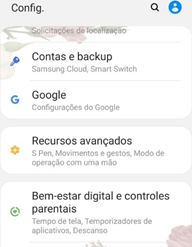
\includegraphics[width=.3\linewidth]{trigonometricas21}
\end{figure}

Por exemplo, alguns registros diários de uso de um aplicativo de mensagens bastante popular no smartphone de uma professora (observando o período de uma semana) estão exibidos a seguir. A primeira informação diz respeito ao número de mensagens recebidas e a segunda informação mostra quantas vezes o aplicativo foi aberto ao longo daquele dia. O dia 13 de agosto foi uma quinta-feira.


\begin{figure}[H]
\centering

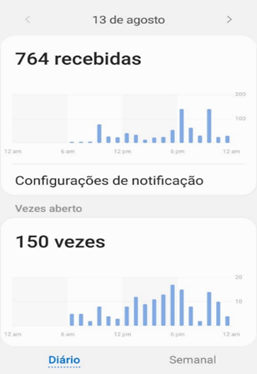
\includegraphics[height=.3\textheight]{trigonometricas22}
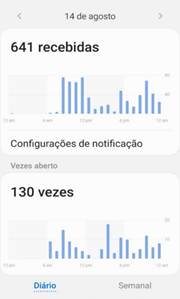
\includegraphics[height=.3\textheight]{trigonometricas23}
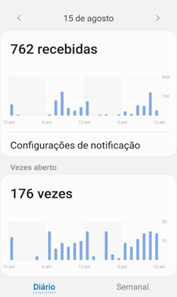
\includegraphics[height=.3\textheight]{trigonometricas24}
\end{figure}

\begin{figure}[H]
\centering

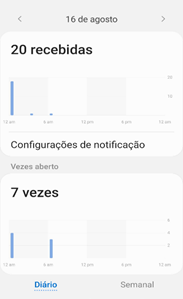
\includegraphics[height=.3\textheight]{trigonometricas25}
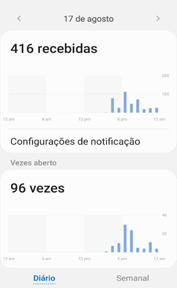
\includegraphics[height=.3\textheight]{trigonometricas26}
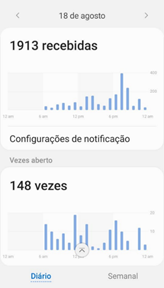
\includegraphics[height=.3\textheight]{trigonometricas27}
\end{figure}

\begin{figure}[H]
\centering

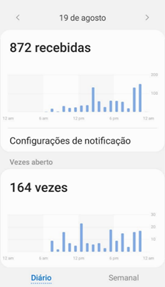
\includegraphics[height=.3\textheight]{trigonometricas28}
\end{figure}
\newpage

\begin{enumerate}
\item Preencha a tabela a seguir com os dados apresentados na figura anterior.

\begin{table}[H]
\centering

\scalebox{.8}
{
\begin{tabular}{|e{.2\linewidth}|e{.2\linewidth}|e{.2\linewidth}|}
\hline
\tcolor{Dia da Semana} & \tcolor{N\super{o} de mensagens recebidas} & \tcolor{N\super{o} de vezes que o aplicativo foi aberto} \tabularnewline
\hline
1 (qui) & & \tabularnewline
\hline
2 (sex) & & \tabularnewline
\hline
3 (sáb) & & \tabularnewline
\hline
4 (dom) & & \tabularnewline
\hline
5 (seg) & & \tabularnewline
\hline
6 (ter) & & \tabularnewline
\hline
7 (qua) & & \tabularnewline
\hline
\end{tabular}
}
\end{table}

\item Marque num plano cartesiano (físico ou digital) pontos $(x,y)$ correspondendo às duas primeiras colunas da tabela, onde $x$ representa o dia da semana e y o número de mensagens recebidas pela professora naquele dia. Em seguida, construa um segmento de reta ligando o ponto correspondente ao dia 1 ao ponto correspondendo ao dia 2, um segmento de reta ligando o ponto correspondente ao dia 2 ao ponto do dia 3 e assim sucessivamente até chegar ao ponto associado ao dia 7.
\item Faça o mesmo que foi pedido no item \titem{b)}, agora considerando que, nos pares $(x,y)$, $x$ representa o dia da semana e $y$ o número de vezes que para a quantidade de vezes em que a professora abre esse aplicativo.
\item Que observações você pode fazer sobre a rotina dessa professora?
\item As funções com domínio sendo o intervalo $[1,7]$ da reta e cujos gráficos foram esboçados nos itens \titem{b)} e \titem{c)} podem ser ditas periódicas? Se sim, justifique; se não, analise as fotos do enunciado de forma a descobrir ao menos algum padrão de regularidade no comportamento da rotina da professora que poderiam dar ideia de periodicidade.
\item Suponha que os mesmos dados de números de mensagens recebidas e de vezes que o aplicativo foi aberto sejam reproduzidos nos dias seguintes: no dia 8, a professora recebe o mesmo número de mensagens que no dia 1, no dia 9 ela recebe o mesmo número de mensagens que no dia 2 e assim sucessivamente (mesmo raciocínio para o número de vezes que o aplicativo foi aberto). As linhas poligonais construídas ligando pontos consecutivos, como feito nos itens \titem{b)} e \titem{c)}, agora representam gráficos de funções periódicas? Se sim, qual será o valor do período e da amplitude delas?
\item Se você ou alguém de sua família tiver um smartphone com essa função, veja que aplicativos aparecem com registro nessa ferramenta e que parâmetros são exibidos (tempo de tela, número de vezes em que o aplicativo é aberto, número de notificações, entre outros).
\item Colete os dados referentes a algum aplicativo de mensagens e anote, reproduzindo os passos \titem{a)}, \titem{b)}, \titem{c)} e \titem{d)}.

\end{enumerate}

\ifdefined\prof
\clearpage
\begin{solucao}

\begin{enumerate}[left=7.5pt, wide]
\item \adjustbox{valign=t}
{
\scalebox{.9}
{
\begin{tabular}{|e{.3\linewidth}|e{.3\linewidth}|e{.3\linewidth}|}
\hline
\tcolor{Dia da Semana} & \tcolor{N\super{o} de mensagens recebidas} & \tcolor{N\super{o} de vezes que o aplicativo foi aberto} \tabularnewline
\hline
1 (qui) & $764$ & $150$ \tabularnewline
\hline
2 (sex) & $641$ & $130$ \tabularnewline
\hline
3 (sáb) & $762$ & $176$ \tabularnewline
\hline
4 (dom) & $20$ & $7$ \tabularnewline
\hline
5 (seg) & $416$ & $96$ \tabularnewline
\hline
6 (ter) & $1913$ & $148$ \tabularnewline
\hline
7 (qua) & $872$ & $164$ \tabularnewline
\hline
\end{tabular}
}
}
\item [\titem{b)} e \titem{c)}] Esses gráficos foram construídos no GeoGebra para Smartphone, a versão Suite GeoGebra
Calculadora, que mescla funções da geometria, da álgebra e planilhas. A função usada foi datafunction({lista de abscissas},{lista de ordenadas}), que associa pontos de um determinado conjunto de dados (se quiser, utilize a opção “Ampliar para enquadrar”{} na Janela de Visualização para conseguir ver a figura como um todo. 

Para o gráfico do número de mensagens por dia da semana, o comando foi 
\begin{center}
\textit{datafunction}($\{1, 2, 3, 4, 5, 6, 7\}, \{764, 641, 762, 20, 416,1913, 872\}$). 
\end{center}
Para o  gráfico do número médio de mensagens por dia da semana, o comando usado foi 
\begin{center}
\textit{datafunction}($\{1, 2, 3, 4, 5, 6, 7\}, \{150, 130, 176, 7, 96, 148, 164\}$).
\end{center}
 Os pontos indicados a seguir foram construídos separadamente, com o objetivo de destacar as informações encontradas na tabela - a saber:
\begin{multicols}{2}
\begin{figure}[H]
\centering
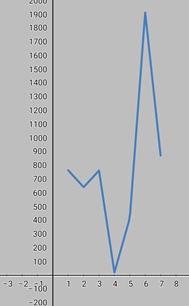
\includegraphics[height=.25\textheight]{trigonometricas29}

\caption{Número de mensagens
recebidas por dia da semana}
\label{}
\end{figure}
\begin{figure}[H]
\centering
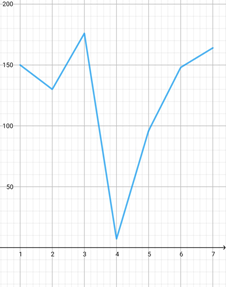
\includegraphics[height=.25\textheight]{trigonometricas30}
\caption{Número de vezes que o
aplicativo foi aberto por dia da semana}
\label{}
\end{figure}
\end{multicols}

\item Há uma queda expressiva nas observações ligadas ao dia 4, que é domingo, o que é natural - tanto em relação ao número de mensagens  ecebidas quanto em relação ao número de vezes que o aplicativo foi aberto. De quarta a sábado observa-se uma queda no número de mensagens recebidas, mas há uma maior ocorrência de abertura do aplicativo. Vale a pena incentivar os alunos a buscar esses dados nos seus próprios smartphones, caso exista essa opção nas configurações, e comparar com as rotinas deles, conforme sugerimos no item \titem{f)}

\item As funções cujos gráficos foram esboçados nos itens b e c não são periódicas, visto a inexistência de um fenômeno cíclico. No entanto, há regularidades que podem ser inferidas a partir da observação das figuras do enunciado, como horários de trabalho - observe que o tempo em que o aplicativo não é aberto é aproximadamente regular ao longo das observações, indicando horário em que a pessoa observada provavelmente está dormindo. Há em geral uma quantidade maior de notificações de mensagens entre os períodos da manhã e tarde, ocorrendo no entanto dias em que isso não se verifica.
\item Podemos construir gráficos que indiquem a reprodução desses trechos ao longo de novas semanas. Dessa forma, o período dessas funções construídas, desses modelos, seria igual a $7$, visto que o trecho encontrado no intervalo de $1$ a $8$ encontra-se “copiado”. Para ilustrar isso,  podemos usar a transformação translação no GeoGebra, ou simplesmente prosseguir marcando os pontos com as mesmas ordenadas e somando $7$ unidades às abscissas, o que gerará uma translação em $7$ unidades para a direita nos dois gráficos. Para usar o GeoGebra, considerando que já temos os gráficos anteriores prontos na tela, podemos construir os pontos $(1,0)$ e $(8,0)$ e construir o vetor com origem em $(1,0)$ e extremidade em $(8,0)$. O vetor está disponível na galeria de comandos “Retas”:



\begin{figure}[H]
\centering

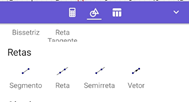
\includegraphics[width=.4\linewidth]{trigonometricas31}
\end{figure}



e então usar a transformação geométrica translação, disponível no menu TRANSFORMAR em Geometria


\begin{figure}[H]
\centering

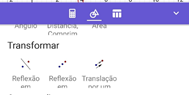
\includegraphics[width=.4\linewidth]{trigonometricas32}
\end{figure}



Ao tocar em translação, precisamos indicar que objeto desejamos transladar e por que vetor. Toque, sequencialmente, após tocar em translação, no gráfico da função e no vetor. Realizando essa mesma sequência novamente de toques a partir sempre da última translação gerada, btemos um gráfico que remete à ideia de uma função periódica. Para a função que representa o número de mensagens recebidas por dia da semana, a amplitude é $\frac{1913−20}{2}= 946{,}5$ e para a função que representa o número de vezes que esse aplicativo foi aberto a cada dia da semana, a amplitude é $\frac{176−7}{2} = 84{,}5$. Para ambas, o período é $8 - 1 = 7$.

Os dois últimos itens são pessoais. Incentive seus alunos a que busquem conhecer melhor sobre essa ferramenta: essa é uma questão de saúde.
\end{enumerate}

\end{solucao}
\fi

\end{document}